\uuid{yAq4}
\exo7id{5118}
\titre{exo7 5118}
\auteur{rouget}
\organisation{exo7}
\datecreate{2010-06-30}
\isIndication{false}
\isCorrection{true}
\chapitre{Injection, surjection, bijection}
\sousChapitre{Bijection}
\module{Algèbre}
\niveau{L1}
\difficulte{}

\contenu{
\texte{
Soit $\begin{array}[t]{cccc}
f~:&\Nn^2&\rightarrow&\Nn\\
 &(x,y)&\mapsto&y+\frac{(x+y)(x+y+1)}{2}
\end{array}$. Montrer que $f$ est une bijection. Préciser, pour $n\in\Nn$ donné, le couple $(x,y)$ dont il est l'image.
}
\reponse{
$f$ est bien une application de $\Nn^2$ dans $\Nn$ car, pour tout couple $(x,y)$ d'entiers
naturels, l'un des deux entiers $x+y$ ou $x+y+1$ est pair et donc, $\frac{(x+y)(x+y+1)}{2}$ est bien un entier naturel
(on peut aussi constater que $\frac{(x+y)(x+y+1)}{2}=1+2+...+(x+y)$ est entier pour $x+y\geq1$).

\textbf{Remarque.} La numérotation de $\Nn^2$ a été effectuée de la façon suivante~:


$$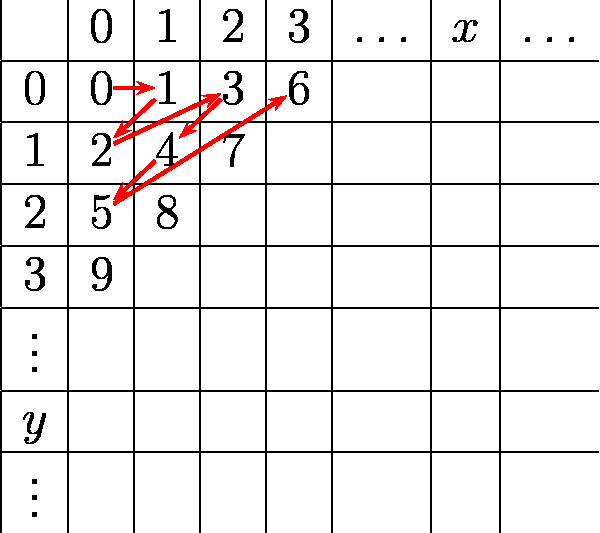
\includegraphics{../images/img005118-1}$$



Sur une parallèle à la droite d'équation $y = -x$, la somme $x+y$ est constante. Il en est de même de l'expression
$\frac{(x+y)(x+y+1)}{2}$ et quand on descend de $1$ en $y$, on avance de $1$ dans la numérotation.

\textbf{Lemme}. $\forall n\in\Nn,\;\exists!p\in\Nn/\;\frac{p(p+1)}{2}\leq n<\frac{(p+1)(p+2)}{2}$.

\textbf{Démonstration}. Pour démontrer ce lemme, on pourrait se contenter de constater que la suite des
nombres triangulaires $\left(\frac{p(p+1)}{2}\right)_{p\geq0}$ est strictement croissante. Néanmoins, on va fournir explicitement
$p$ en fonction de $n$.
Soient $n$ et $p$ deux entiers naturels.
\begin{align*}
\frac{p(p+1)}{2}\leq n<\frac{(p+1)(p+2)}{2}&\Leftrightarrow p^2+p-2n\leq0\;\mbox{et}\;p^2+3p+2-2n>0\\
 &\Leftrightarrow p\leq\frac{-1+\sqrt{8n+1}}{2}\;\mbox{et}\;p>\frac{-3+\sqrt{8n+1}}{2}=-1+\frac{-1+\sqrt{8n+1}}{2}\\
 &\Leftrightarrow p\leq\frac{-1+\sqrt{8n+1}}{2}<p+1\Leftrightarrow p= E\left(\frac{-1+\sqrt{8n+1}}{2}\right).
\end{align*}
Le lemme est démontré.

Montrons que $f$ est surjective (et au passage, déterminons l'antécédent d'un entier $n$ donné).
Soient $n$ un entier naturel et $p=E\left(\frac{-1+\sqrt{8n+1}}{2}\right)$ ($p$ est un entier naturel). On pose $\left\{
\begin{array}{l}
x+y=p\\
y=n-\frac{p(p+1)}{2}
\end{array}
\right.$ ou encore $\left\{
\begin{array}{l}
y=n-\frac{p(p+1)}{2}\\
x=p-y=\frac{p(p+3)}{2}-n
\end{array}
\right.$. Tout d'abord, $y+\frac{(x+y)(x+y+1)}{2}=n-\frac{p(p+1)}{2}+\frac{p(p+1)}{2}=n$. Mais il reste encore à
vérifier que $x$ et $y$ ainsi définis (qui sont à l'évidence des entiers relatifs) sont bien des entiers
naturels. Puisque $\frac{p(p+1)}{2}$ est un entier naturel et que $n\geq\frac{p(p+1)}{2}$, $y$ est bien un entier
naturel. Ensuite, $\frac{p(p+3)}{2}=\frac{p(p+1)}{2}+p$ est aussi un entier naturel et de plus,

$$\frac{p(p+3)}{2}-n\geq\frac{p(p+3)}{2}-\left(\frac{(p+1)(p+2)}{2}-1\right)=0,$$
et $x$ est bien un entier naturel. Ainsi, pour $n$ naturel donné, en posant $p= E\left(\frac{-1+\sqrt{8n+1}}{2}\right)$ puis
$x=\frac{p(p+3)}{2}-n$ et $y=n-\frac{p(p+1)}{2}$, $x$ et $y$ sont des entiers naturels tels que $f((x,y))=n$. $f$ est
donc surjective.
Montrons que $f$ est injective.
Pour cela, on montre que si $x$ et $y$ sont des entiers naturels vérifiant
$y+\frac{(x+y)(x+y+1)}{2}=n$, alors nécessairement, $x+y=p$ (et $y=n-\frac{p(p+1)}{2})$.
Soient donc $x$ et $y$ deux entiers naturels. On a~:

$$\frac{(x+y)(x+y+1)}{2}\leq\frac{(x+y)(x+y+1)}{2}+y=n<\frac{(x+y)(x+y+1)}{2}+(x+y+1)=\frac{(x+y+1)(x+y+2)}{2},$$
et le lemme montre que $x+y=p$. L'unicité du couple $(x,y)$ est donc démontrée. $f$ est une application injective et
surjective et donc $f$ est bijective. Sa réciproque est $\begin{array}[t]{cccc}
f^{-1}~:&\Nn&\rightarrow&\Nn^2\\
 &n&\mapsto&(\frac{p(p+3)}{2}-n,n-\frac{p(p+1)}{2})
\end{array}$ où $p=E\left(\frac{-1+\sqrt{8n+1}}{2}\right)$.
}
}
